% !TEX program = xelatex

\documentclass[a4paper,UTF8]{article}
\usepackage{ctex}
\usepackage[margin=1.25in]{geometry}
\usepackage{color}
\usepackage{graphicx}
\usepackage{amssymb}
\usepackage{amsmath}
\usepackage{amsthm}
\usepackage{enumerate}
\usepackage{bm}
\usepackage{hyperref}
\usepackage{epsfig}
\usepackage{color}
\usepackage{tcolorbox}
\usepackage{mdframed}
\usepackage{lipsum}
\usepackage{epsfig}
\usepackage{graphicx}
\usepackage{subfigure}
\usepackage{float}
\newmdtheoremenv{thm-box}{myThm}
\newmdtheoremenv{prop-box}{Proposition}
\newmdtheoremenv{def-box}{定义}

\setlength{\evensidemargin}{.25in}
\setlength{\textwidth}{6in}
\setlength{\topmargin}{-0.5in}
\setlength{\topmargin}{-0.5in}
% \setlength{\textheight}{9.5in}
%%%%%%%%%%%%%%%%%%此处用于设置页眉页脚%%%%%%%%%%%%%%%%%%
\usepackage{fancyhdr}                                
\usepackage{lastpage}                                           
\usepackage{layout}                                             
\footskip = 10pt 
\pagestyle{fancy}                    % 设置页眉                 
\lhead{2018年春季}                    
\chead{机器学习导论}                                                
% \rhead{第\thepage/\pageref{LastPage}页} 
\rhead{作业一}                                                                                               
\cfoot{\thepage}                                                
\renewcommand{\headrulewidth}{1pt}  			%页眉线宽,设为0可以去页眉线
\setlength{\skip\footins}{0.5cm}    			%脚注与正文的距离           
\renewcommand{\footrulewidth}{0pt}  			%页脚线宽,设为0可以去页脚线

\makeatletter 									%设置双线页眉                                        
\def\headrule{{\if@fancyplain\let\headrulewidth\plainheadrulewidth\fi%
\hrule\@height 1.0pt \@width\headwidth\vskip1pt	%上面线为1pt粗  
\hrule\@height 0.5pt\@width\headwidth  			%下面0.5pt粗            
\vskip-2\headrulewidth\vskip-1pt}      			%两条线的距离1pt        
 \vspace{6mm}}     								%双线与下面正文之间的垂直间距              
\makeatother  

%%%%%%%%%%%%%%%%%%%%%%%%%%%%%%%%%%%%%%%%%%%%%%
\numberwithin{equation}{section}
%\usepackage[thmmarks, amsmath, thref]{ntheorem}
\newtheorem{myThm}{myThm}
\newtheorem*{myDef}{Definition}
\newtheorem*{mySol}{Solution}
\newtheorem*{myProof}{Proof}
\newcommand{\indep}{\rotatebox[origin=c]{90}{$\models$}}
\newcommand*\diff{\mathop{}\!\mathrm{d}}

\usepackage{multirow}

%--

%--
\begin{document}
\title{机器学习导论\\
作业一}
\author{151220129, 吴政亿, 18805156360@163.com}
\maketitle

\section*{学术诚信}

本课程非常重视学术诚信规范,助教老师和助教同学将不遗余力地维护作业中的学术诚信规范的建立。希望所有选课学生能够对此予以重视。\footnote{参考尹一通老师\href{http://tcs.nju.edu.cn/wiki/}{高级算法课程}中对学术诚信的说明。}

\begin{tcolorbox}
\begin{enumerate}
  \item[(1)] 允许同学之间的相互讨论,但是{\color{red}\textbf{署你名字的工作必须由你完成}},不允许直接照搬任何已有的材料,必须独立完成作业的书写过程;
  \item[(2)] 在完成作业过程中,对他人工作(出版物、互联网资料)中文本的直接照搬(包括原文的直接复制粘贴及语句的简单修改等)都将视为剽窃,剽窃者成绩将被取消。{\color{red}\textbf{对于完成作业中有关键作用的公开资料,应予以明显引用}};
  \item[(3)] 如果发现作业之间高度相似将被判定为互相抄袭行为,{\color{red}\textbf{抄袭和被抄袭双方的成绩都将被取消}}。因此请主动防止自己的作业被他人抄袭。
\end{enumerate}
\end{tcolorbox}

\section*{作业提交注意事项}
\begin{tcolorbox}
\begin{enumerate}
  \item[(1)] 请严格参照课程网站作业提交方法一节提交作业;
  \item[(2)] 未按照要求提交作业,或提交作业格式不正确,将会被扣除部分作业分数;
  \item[(3)] 除非有特殊情况(如因病缓交),否则截止时间后不接收作业,本次作业记零分。
\end{enumerate}
\end{tcolorbox}

\newpage
\section{[25pts] Basic Probability and Statistics}
随机变量$X$的概率密度函数如下,
\begin{equation}
	f_X(x) = 
	\begin{cases}
		\frac{1}{4} & 0<x<1;\\
		\frac{3}{8} & 3<x<5;\\
		0			& \mbox{otherwise.}
	\end{cases}
\end{equation}
\begin{enumerate}[ {(}1{)}]
\item \textbf{[5pts]} 请计算随机变量$X$的累积分布函数$F_X(x)$;
\item \textbf{[10pts]} 随机变量$Y$定义为$Y = 1/X$,求随机变量$Y$对应的概率密度函数$f_Y(y)$;
\item \textbf{[10pts]} 试证明,对于非负随机变量$Z$,如下两种计算期望的公式是等价的。
\begin{equation}
	\label{eq-expect-1}
	\mathbb{E}[Z] = \int_{z=0}^{\infty}zf(z) \diff z.
\end{equation}

\begin{equation}
	\label{eq-expect-2}
	\mathbb{E}[Z] = \int_{z=0}^{\infty}\Pr[Z\geq z] \diff z.
\end{equation}

同时,请分别利用上述两种期望公式计算随机变量$X$和$Y$的期望,验证你的结论。
\end{enumerate}
\begin{mySol}
此处用于写解答(中英文均可)

答:
\begin{enumerate}[ {(}1{)}]
\item 
\begin{eqnarray*}
	F_X(x) = 
	\begin{cases}
		0				& x \leq 0 \\
		\frac{1}{4} x 	& 0<x<1;\\
		\frac{1}{4} 	& 1 \leq x \leq 3;\\
		\frac{3}{8} x - \frac{7}{8} & 3<x<5;\\
		1				& x \geq 5 
	\end{cases}
\end{eqnarray*}

\item 
\begin{eqnarray*}
	&F_Y(y)&=Pr[Y<y]=Pr[1/X<y]\\
	&&=1-Pr[X<1/y]=1-F_X(1/y)\\
	&&=
	\begin{cases}
		0				& y \leq \frac{1}{5} \\
		\frac{15}{8}-\frac{3}{8y} &\frac{1}{5}<y<\frac{1}{3};\\
		\frac{3}{4} 	& \frac{1}{3} \leq y \leq 1;\\
		1 - \frac{1}{4y} & 1<y;
	\end{cases}
	\\
	&f_Y(y) = F_Y'(y) &= 
	\begin{cases}
		\frac{3}{8y^2} & \frac{1}{5}<y<\frac{1}{3};\\
		\frac{1}{4y^2} & 1<y;\\
		0					& \mbox{otherwise.}
	\end{cases}
\end{eqnarray*}

\item
\begin{eqnarray*}
	\int^{\infty}_{z=0}{Pr[Z \geq z]dz} 
		&&= \int^{\infty}_{z=0}\int^{\infty}_{z}{f(t)dtdz}\\
		&&= \int^{\infty}_{t=0}\int^t_0{f(t)}dzdt\\
		&&= \int^{\infty}_{t=0}{tf(t)}dt\\
		&&= \int^{\infty}_{z=0}{zf(z)}dz\\
	\\	
	E[X]&&=\int^{\infty}_{z=0}{zf(z)}dz\\
		&&=\int^{1}_{0}{\frac14 z}dz +\int^{5}_{3}{z\frac38}dz\\
		&&=\frac{1}{8} + 3 = \frac{25}{8}\\	
	\\
	E[X]&&=\int^{\infty}_{z=0}{Pr[Z \geq z]dz} \\
		&&=\int^{1}_{0}{(1-\frac{1}{4}x)dx}
		+\int^{3}_{1}{\frac{3}{4}dx}
		+\int^{5}_{3}{(\frac{15}{8}-\frac{3}{8}x)dx}
		+\int^{\infty}_{5}{0dx}\\
		&&=\frac{7}{8}+\frac{3}{2}+\frac{3}{4}+0
		=\frac{25}{8}\\
	\\
	E[Y]&&=\int^{\infty}_{z=0}{zf(z)}dz\\
		&&=\int^{\frac{1}{3}}_{\frac{1}{5}}{\frac{3}{8y^2}}dy 
		+\int^{\infty}_{1}{\frac{1}{4y} dy}\\
		&&=\frac{3}{4}+ \infty
	\\
	E[Y]&&=\int^{\infty}_{z=0}{Pr[Z \geq z]dz} \\
		&&=\int^{\frac{1}{5}}_{0}{dy}
		+\int^{\frac{1}{3}}_{\frac{1}{5}}{(\frac{3}{8y}-\frac{7}{8})dy}
		+\int^{1}_{\frac{1}{3}}{(\frac{1}{4})dy}
		+\int^{\infty}_{1}{(1-\frac{1}{4y})dy}\\
		&&=...-\int^{\infty}_{1}{(\frac{1}{4y})dy}\\
		&&=-\infty\\
\end{eqnarray*}
	所以$E[X]=\frac{25}{8},E[Y]$不存在。
\end{enumerate}

\end{mySol}

\newpage

\section{[20pts] Strong Convexity}
通过课本附录章节的学习,我们了解到凸性(convexity)对于机器学习的优化问题来说是非常良好的性质。下面,我们将引入比凸性还要好的性质——强凸性(strong convexity)。
\begin{def-box}[强凸性]
记函数$f: \mathcal{K} \rightarrow \mathbb{R}$,如果对于任意$\mathbf{x}, \mathbf{y} \in \mathcal{K}$及任意$\alpha\in[0,1]$,有以下命题成立
\begin{equation}
  \label{eq-sc-1}
  f((1-\alpha)\mathbf{x} + \alpha\mathbf{y})\leq (1-\alpha)f(\mathbf{x}) + \alpha f(\mathbf{y}) - \frac{\lambda}{2}\alpha(1-\alpha)\lVert \mathbf{x} - \mathbf{y}\rVert^2.
\end{equation}
则我们称函数$f$为关于范数$\lVert \cdot \rVert$的$\lambda$-强凸函数。
\end{def-box}

请证明,在函数$f$可微的情况下,式~\eqref{eq-sc-1}与下式~\eqref{eq-sc-2}等价,
\begin{equation}
  \label{eq-sc-2}
  f(\mathbf{y}) \geq f(\mathbf{x}) + \nabla f(\mathbf{x})^\mathrm{T}(\mathbf{y}-\mathbf{x}) + \frac{\lambda}{2}\lVert \mathbf{y} - \mathbf{x}\rVert^2.
\end{equation}
\begin{myProof}
此处用于写证明(中英文均可)
~\\
~\\
答:\\
\begin{enumerate}
\item[(1)]$\ref{eq-sc-1} \Leftarrow \ref{eq-sc-2}$\\
设$\mathbf{z}=(1-\alpha)\mathbf{x}+\alpha \mathbf{y}$
,由\ref{eq-sc-2}有:\\
\begin{equation}
  \label{eq-sc-3}
  f(\mathbf{x}) \geq f(\mathbf{z}) + \nabla f(\mathbf{z})^\mathrm{T}(\mathbf{x}-\mathbf{z}) + \frac{\lambda}{2}\lVert \mathbf{x} - \mathbf{z}\rVert^2.
\end{equation}

\begin{equation}
  \label{eq-sc-4}
  f(\mathbf{y}) \geq f(\mathbf{z}) + \nabla f(\mathbf{z})^\mathrm{T}(\mathbf{y}-\mathbf{z}) + \frac{\lambda}{2}\lVert \mathbf{y} - \mathbf{z}\rVert^2.
\end{equation}
$(1-\alpha)$\ref{eq-sc-3} $+ \alpha$\ref{eq-sc-4}得到\\
\begin{eqnarray*}
  (1-\alpha)f(\mathbf{x})+\alpha f(\mathbf{y}) 
  \geq f(\mathbf{z}) 
  + \nabla f(\mathbf{z})^\mathrm{T}((1-\alpha)\mathbf{x}+\alpha\mathbf{y}-\mathbf{z}) 
  + \frac{\lambda(1-\alpha)}{2}\lVert \mathbf{x} - \mathbf{z}\rVert^2 
  + \frac{\lambda\alpha}{2}\lVert \mathbf{y} - \mathbf{z}\rVert^2.
\end{eqnarray*}
\begin{eqnarray*}
  f(\mathbf{z})
  &&\leq (1-\alpha)f(\mathbf{x})+\alpha f(\mathbf{y})
  - \nabla f(\mathbf{z})^\mathrm{T}((1-\alpha)\mathbf{x}+\alpha\mathbf{y}-\mathbf{z})
  - \frac{\lambda(1-\alpha)}{2}\lVert \mathbf{x}
  - \mathbf{z}\rVert^2 - \frac{\lambda\alpha}{2}\lVert \mathbf{y} - \mathbf{z}\rVert^2.\\
  &&\leq (1-\alpha)f(\mathbf{x})+\alpha f(\mathbf{y})
  - \frac{\lambda(1-\alpha)}{2}\lVert \mathbf{x}- \mathbf{z}\rVert^2 
  - \frac{\lambda\alpha}{2}\lVert \mathbf{y} - \mathbf{z}\rVert^2.\\
  &&\leq (1-\alpha)f(\mathbf{x})+\alpha f(\mathbf{y})
  - \frac{\lambda(1-\alpha)}{2}\lVert \alpha(\mathbf{x}- \mathbf{y})\rVert^2 
  - \frac{\lambda\alpha}{2}\lVert (1-\alpha)(\mathbf{y} - \mathbf{x})\rVert^2.\\
  &&\leq (1-\alpha)f(\mathbf{x})+\alpha f(\mathbf{y})
  - \frac{\lambda(1-\alpha)\alpha^2}{2}\lVert \mathbf{x}- \mathbf{y}\rVert^2 
  - \frac{\lambda\alpha (1-\alpha)^2}{2}\lVert \mathbf{y} - \mathbf{x} \rVert^2.\\
  &&\leq (1-\alpha)f(\mathbf{x})+\alpha f(\mathbf{y})
  - \frac{\lambda(1-\alpha)\alpha}{2}\lVert \mathbf{x}- \mathbf{y}\rVert^2.
\end{eqnarray*}
代入$\mathbf{z}=(1-\alpha)\mathbf{x}+\alpha \mathbf{y}$得到:\\
\begin{eqnarray*}
  f((1-\alpha)\mathbf{x} + \alpha\mathbf{y})\leq (1-\alpha)f(\mathbf{x}) + \alpha f(\mathbf{y}) - \frac{\lambda}{2}\alpha(1-\alpha)\lVert \mathbf{x} - \mathbf{y}\rVert^2.
\end{eqnarray*}

\item[(2)]$\ref{eq-sc-1} \Rightarrow \ref{eq-sc-2}$\\
\begin{eqnarray*}
  f((1-\alpha)\mathbf{x} + \alpha\mathbf{y})
  &&\leq (1-\alpha)f(\mathbf{x}) + \alpha f(\mathbf{y}) 
  - \frac{\lambda}{2}\alpha(1-\alpha)\lVert \mathbf{x} - \mathbf{y}\rVert^2.\\
  f(\mathbf{x} + \alpha(\mathbf{y}-\mathbf{x}))
  &&\leq f(\mathbf{x}) + \alpha (f(\mathbf{y}) -f(\mathbf{x}))
  - \frac{\lambda}{2}\alpha(1-\alpha)\lVert \mathbf{x} - \mathbf{y}\rVert^2.\\
  f(\mathbf{y}) -f(\mathbf{x})
  &&\geq \frac{f(\mathbf{x} + \alpha(\mathbf{y}-\mathbf{x}))-f(\mathbf{x})}{a}
  +  \frac{\lambda}{2}(1-\alpha)\lVert \mathbf{x} - \mathbf{y}\rVert^2.\\
  when \alpha \rightarrow 0\\
  f(\mathbf{y}) -f(\mathbf{x})
  &&\geq \nabla f(\mathbf{x})^\mathrm{T}(\mathbf{y}-\mathbf{x}) 
  + \frac{\lambda}{2}\lVert \mathbf{y} - \mathbf{x}\rVert^2.\\
  f(\mathbf{y}) 
  &&\geq f(\mathbf{x}) 
  + \nabla f(\mathbf{x})^\mathrm{T}(\mathbf{y}-\mathbf{x}) 
  + \frac{\lambda}{2}\lVert \mathbf{y} - \mathbf{x}\rVert^2.
\end{eqnarray*}
问题得证。

\end{enumerate}
\qed
\end{myProof}


\newpage
\section{[20pts] Double Stochastic Matrix}
随机矩阵(stochastic matrix)和双随机矩阵(double stochastic matrix)在机器学习中经常出现,尤其是在有限马尔科夫过程理论中,也经常出现在于运筹学、经济学、交通运输等不同领域的建模中。下面给出定义,
\begin{def-box}[随机矩阵]
设矩阵$\mathbf{X}=[x_{ij}]\in \mathbb{R}^{d\times d}$是非负矩阵,如果$\mathbf{X}$满足
\begin{equation}
	\label{eq-sto-matrix}
	\sum_{j=1}^d x_{ij} = 1,\quad i=1,2,\cdots,d.
\end{equation}
则称矩阵$\mathbf{X}$为随机矩阵(stochastic matrix)。如果$\mathbf{X}$还满足
\begin{equation}
	\label{eq-double-sto-matrix}
	\sum_{i=1}^d x_{ij} = 1,\quad j=1,2,\cdots,d.
\end{equation}
则称矩阵$\mathbf{X}$为双随机矩阵(double stochastic matrix)。
\end{def-box}
对于双随机矩阵$\mathbf{X} \in \mathbb{R}^{d\times d}$,试证明
\begin{enumerate}[ {(}1{)}]
\item \textbf{[10pts]} 矩阵$\mathbf{X}$的\href{https://en.wikipedia.org/wiki/Entropy_(information_theory)}{信息熵 (entropy)}满足$H(\mathbf{X}) \leq d\log d$.
\item \textbf{[10pts]} 矩阵$\mathbf{X}$的\href{https://en.wikipedia.org/wiki/Spectral_radius}{谱半径 (spectral radius
)}$\rho(\mathbf{X})$等于1,且是$\mathbf{X}$的特征值;(提示:你可能会需要\href{https://en.wikipedia.org/wiki/Perron%E2%80%93Frobenius_theorem}{Perron–Frobenius定理},可以基于此进行证明。)
\end{enumerate}
\begin{myProof}
此处用于写证明(中英文均可)
~\\
~\\
答:\\
\begin{enumerate}[ {(}1{)}]
\item
\begin{eqnarray*}
	&H(X)&= -\sum_{i=1}^{d}\sum_{j=1}^{d}{D_{ij}\log{X_{ij}}}\\
		 &&= -\sum_{i=1}^{d}(\sum_{j=1}^{d}{D_{ij}\log{X_{ij}}})\\
	&\because &(x\log{x})'' > 0\\
	&\therefore &{\frac{\sum_{x_i}}{n}}\log{{\frac{\sum_{x_i}}{n}}} 
				\leq \frac{1}{n}\sum{x_i\log{x_i}}\\
	&\therefore &H(x) \leq -\sum_{i=1}^{d}
	{(d*\frac{1}{d}\log{\frac{1}{d}})}=d\log{d}
\end{eqnarray*}
\item

\end{enumerate}

\qed
\end{myProof}
\newpage
\section{[15pts] Hypothesis Testing} 
在数据集$D_1,D_2,D_3,D_4,D_5$运行了$A,B,C,D,E$五种算法,算法比较序值表如表\ref{table:ranking}所示:
\begin{table}[h]
\centering
\caption{算法比较序值表} \vspace{2mm}
\label{table:ranking}
\begin{tabular}{c|c c c c c}\hline
数据集 		& 算法$A$  	&算法$B$  	& 算法$C$ 	& 算法$D$  	&算法$E$ 	\\ \hline
$D_1$ 		& 4 		&  3  		& 5  		&  2 		& 1			\\
$D_2$ 		& 3 		&  5  		& 2  		&  1 		& 4			\\
$D_3$ 		& 4 		&  5  		& 3  		&  1 		& 2			\\ 
$D_4$ 		& 5 		&  2  		& 4  		&  1 		& 3			\\ 
$D_5$ 		& 3 		&  5  		& 2  		&  1 		& 4			\\ \hline
\end{tabular}
\end{table}

使用Friedman检验$(\alpha=0.05)$判断这些算法是否性能都相同。若不相同,进行Nemenyi后续检验$(\alpha=0.05)$,并说明性能最好的算法与哪些算法有显著差别。
\begin{mySol}
此处用于写解答(中英文均可)
~\\
~\\
答:\\
~\\
查表得当$\alpha = 0.05$,数据集个数$N = 5$,算法个数$k = 5$时,F检验常用临界值为3.007\\
计算得算法A到E的平均序值为$3.8,4,3.2,1.2,2.8$\\
\[
\tau_{\chi^2} 
= \frac{12N}{k(k+1)}(\sum^k_{i=1}{r_i^2}-\frac{k(k+1)^2}{4})
=\frac{12*5}{5(6)}(3.8^2+4^2+3.2^2+1.2^2+2.8^2-\frac{5(6)^2}{4})
=9.92
\]
\[
\tau_F 
= \frac{(N-1)\tau_{\chi^2}}{N(k-1)-\tau_{\chi^2}}
= \frac{4*9.92}{5*4-9.92}
= 3.9365 > 3.007 
\]
因此拒绝“所有算法性能相同”这个假设。下面进行Nemenyi后续检验:\\
查表得当$\alpha = 0.05$,数据集个数$N = 5$,算法个数$k = 5$时,
$q_{0.05}=2.728$\\
\[CD 	= q_{\alpha}\sqrt{\frac{k(k+1)}{6N}}
		= 2.728*\sqrt{\frac{5*6}{6*5}}
		= 2.728
		\]
由计算的平均序值可知,只有算法B与算法D的差距超过临界值域,因此检验结果认为算法B与算法D的性能显著不同,而其他两两之间的性能没有显著差别。
\end{mySol}

\newpage
\section{[20pts] ROC and AUC}
现在有五个测试样例,其对应的真实标记和学习器的输出值如表\ref{table:roc}所示:
\begin{table}[!h]
	\centering
	\caption{测试样例表} \vspace{2mm}\label{table:roc}
	\begin{tabular}{c|c c c c c}\hline
		样本 & $x_1$ & $x_2$ & $x_3$  & $x_4$  & $x_5$ \\
		\hline
		标记 & +  & + &  - &  +  & -\\
		\hline
		输出值 & 0.9  & 0.3 &  0.1 &  0.7  & 0.4\\
		\hline
	\end{tabular}
\end{table}
\begin{enumerate}[ {(}1{)}]
\item \textbf{[10pts]} 请画出其对应的ROC图像,并计算对应的$\mbox{AUC}$和$\ell_{rank}$的值(提示:可使用\href{https://en.wikibooks.org/wiki/LaTeX/PGF/TikZ}{TikZ包}作为\LaTeX 中的画图工具);
\item \textbf{[10pts]} 根据书上第35页中的公式(2.20)和公式(2.21),试证明\[\mbox{AUC}+\ell_{rank}=1.\]
\end{enumerate}
\begin{mySol}
此处用于写解答(中英文均可)
~\\
答:\\

\begin{enumerate}[ {(}1{)}]
\item 
	根据预测结果与样例进行排序,则分别为 + + - + -。\\
	计算得$\frac{1}{m^+}=\frac{1}{3},\frac{1}{m^-}=\frac{1}{2}$
	则他们的坐标分别为
	
	\begin{eqnarray*}
	(0,0),
	(0,\frac{1}{3}),
	(0,\frac{2}{3}),
	(\frac{1}{2},\frac{2}{3}),
	(\frac{1}{2},1),
	(1,1)
	\end{eqnarray*}
	
	ROC图像为:\\
	
	\begin{figure}[H]
	\begin{center}
		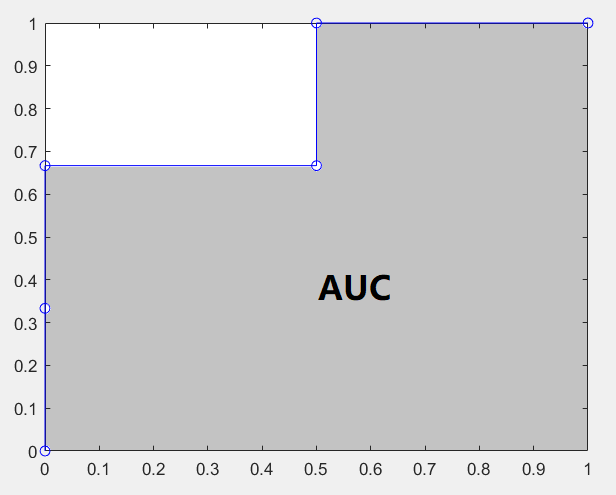
\includegraphics[width=0.32\linewidth]{roc.png}
		%\caption{An image of Lena.}
		%\label{Fig:1}
	\end{center}
	\vspace{-0.5em}
	\end{figure}
	
	\[
		AUC=\frac{1}{2}\sum^{m-1}_{i=1}{(x_{i+1}-x_i)*(y_i+y_{i+1})}
		=\frac{1}{2}*(\frac{1}{2}*\frac{4}{3}+\frac{1}{2}*1)
		=\frac{7}{12}		
	\] 
	\[\ell_{rank}=1-AUC=\frac{5}{12}\]
	
\item
	根据ROC曲线的绘制,计算AUC时,考虑每一对正、反例,若正例的预测值小于反例,则x先增加,y后增加,AUC不会增加;若正例的预测值大于反例,则y先增加,x后增加,AUC增加$\frac{1}{m^+m^-}$;若正例的预测值等于反例,则x,y同时增加,AUC增加$\frac{1}{2m^+m^-}$。\\
	
	\[
	\therefore AUC=\frac{1}{m^+m^-}\sum_{x^+ \in D^+}\sum_{x^- \in D^-}(I(f(x^+)>f(x^-))+\frac{1}{2}I(f(x^+)=f(x^-)))
	\]
	
	\[
	\because \ell_{rank}=\frac{1}{m^+m^-}\sum_{x^+ \in D^+}\sum_{x^- \in D^-}(I(f(x^+)<f(x^-))+\frac{1}{2}I(f(x^+)=f(x^-)))
	\]
	
	\[\therefore AUC+\ell_{rank}=1 \]
	
\end{enumerate}

\end{mySol}

\newpage
\section{[附加题10pts] Expected Prediction Error}
对于最小二乘线性回归问题,我们假设其线性模型为:
\begin{equation}
	y=\textbf{x}^T  \bm{ \beta } + \epsilon , 
\end{equation}
其中$\epsilon$为噪声满足$\epsilon\sim N(0,\sigma^2)$。我们记训练集$\mathcal{D}$中的样本特征为$\textbf{X}\in \mathbb{R}^{p \times n}$,标记为$\textbf{Y}\in \mathbb{R}^{n}$,其中$n$为样本数,$p$为特征维度。
已知线性模型参数的估计为:
\begin{equation}
	\hat{\bm{\beta}}=(\textbf{X}\textbf{X}^T)^{-1}\textbf{X}\textbf{Y}.	
\end{equation}

对于给定的测试样本$\textbf{x}_0$,记$\mathbf{EPE}(\textbf{x}_0)$为其预测误差的期望 (Expected Predication Error),试证明,
\[
	\mathbf{EPE}(\textbf{x}_0) = \sigma^2+\mathbb{E}_{\mathcal{D}}[\textbf{x}_0^T(\textbf{X}\textbf{X}^T)^{-1}\textbf{x}_0\sigma^2].
\]

要求证明中给出详细的步骤与证明细节。(提示:$\mathbf{EPE}(\textbf{x}_0)=\mathbb{E}_{y_0|\textbf{x}_0} \mathbb{E}_{\mathcal{D}}[(y_0-\hat{y}_0)^2]$,可以参考书中第45页关于方差-偏差分解的证明过程。)

\begin{myProof}
此处用于写证明(中英文均可)
~\\
~\\
~\\
~\\
~\\
\qed
\end{myProof}




\end{document}
